\chapter{极小曲面的基本性质}
极小曲面起源于下面的问题:
\begin{question*}
    给定简单闭曲线$\gamma \subset \R^3$, 是否存在以$\gamma$为边界的面积最小的曲面? 即, 寻找曲面$\Sigma, \partial \Sigma = \gamma$, 使得对于任意满足$\partial \Sigma' = \gamma$的曲面$\Sigma'$, 都有
    \begin{equation*}
        \Area(\Sigma) \le \Area(\Sigma')
    \end{equation*}
\end{question*}
这个问题现在被称为Plateau问题(虽然它最早由Langrage提出). 1920-30s年代, 这个问题被Rado和Douglas解决(Douglas也因为在Plateau上的工作而获得第一届Fields奖).
\section{极小曲面方程}
每个曲面都可以局部地表示为函数的图像的形式, 因此我们首先来研究可以作为函数图像的曲面. 设$\Sigma$是面积最小的曲面, 且
\begin{equation*}
    \Sigma= \G(u)= \{(x,u(x))\mid x \in \Omega\}
\end{equation*}
其中, $\Omega$ 是给定的有界区域, $u \in \CC(\Omega)$. 由于$\G(u)$面积最小, 那么对于任意$\phi \in \CC(\Omega)$ 及$t \in \R$,
\begin{equation}
    \Area(\G(u)) \le \Area(\G(u+t\phi))
\end{equation}
于是, 我们有
\begin{equation}
    \ddt(\Area(\G(u+t\phi)))\mid {t=0}=0
\end{equation}
直接计算可知
\begin{equation}
    \begin{split}
        \Area(\G(u+t\phi)) &= \int_\Omega \sqrt{1+\abs{Du+tD\phi}^2} \\
                          &= \int_\Omega \sqrt{1+\abs{Du}^2}+t\frac{\inner{Du}{D\phi}}{\sqrt{1+\abs{Du}^2}} + o(t)
    \end{split}
\end{equation}
因此, $\forall \phi \in \CC(\Omega)$, 成立
\begin{equation}
    \begin{split}
        \ddt \Area(\G(u+t\phi))\mid _{t=0} & = \int_\Omega \frac{\inner{Du}{D\phi}}{\sqrt{1+\abs{Du}^2}} \\
        &=- \int_\Omega \phi \div \frac{Du}{\sqrt{1+\abs{Du}^2}} =0
    \end{split}
\end{equation}
下面的方程便称为极小曲面方程(MSE).
\begin{equation}
    \div \frac{Du}{\sqrt{1+\abs{Du}^2}} =0
\end{equation}
\begin{remark}
    一个曲面是否局部地满足MSE, 跟我们选取的坐标表示是没有关系的.
\end{remark}
显然地, 一个函数$u$满足极小曲面方程只是$\G(u)$面积最小的必要条件, 是否有可能是充分条件? 我们有下面的两个结论.
\begin{proposition}\label{mse_min1}
    设$\Omega \subset \R^n$是有界区域, $u \in C^2(\Omega)\cap C(\overline{\Omega})$. 设$u$满足MSE. 设$\Sigma \subset \Omega \times \R$且$\partial \Sigma = \partial \G(u)$. 则有
    \begin{equation}
        \Area(\G(u)) \le \Area(\Sigma)
    \end{equation}
\end{proposition}
\begin{proof}
    记$\vec{n}= \frac{\partial_{n+1}-Du}{\sqrt{1+\abs{Du}^2}}$为$\G(u)$的单位法向(这里我们将$\vec{n}$自然地扩张到$\R^{n+1}$上). 由于$u$满足MSE, 则$\div(\vec{n})=0$. 设$dx$是$\R^{n+1}$中的体积形式, 定义$n-$ 形式 $\omega=i_*^{\vec{n}}dx$如下, 对于任意向量场 $X_1,X_2, \cdots,X_n$:
    \begin{equation}
        \omega(X_1,X_2,\cdots,X_n)=dx(X_1,X_2,\cdots,X_n,\vec{n})
    \end{equation}
    显然地, $\omega$是多重线性的反对称张量, 即是一个$n-$形式.  现在验证$\omega$有如下性质:
    \begin{enumerate}
        \item $d\omega=0$.
        \item $\forall$ 单位向量场 $e_1,e_2,\cdots,e_n$, 成立$\omega(e_1,e_2,\cdots,e_n) \le 1$. 并且等号成立当且仅当$e_1,e_2,\cdots,e_n$形成$T\Sigma$的标准正交基.
    \end{enumerate}
    性质(1)由基本公式$d(i_*^{\vec{n}}dx)=\div(\vec{n})dx$ 可知.  为了验证性质 (2), 设$V=span(e_2,e_3,\cdots,e_n,\vec{n})$. 将$e_1$分解为平行于$V$和垂直于$V$的部分, $e_1=e_1^T+e_1^{\perp}$. 则
    \begin{equation}
        \omega(e_1,\cdots,e_n,\vec{n})=\det([e_1^{\perp}, e_2,\cdots,e_n,\vec{n}])
    \end{equation}
    同样的相对于空间$span(e_3,\cdots,e_n,\vec{n})$, 分解$e_2$. 这样一直做下去, 最终有
    \begin{equation}
        \omega(e_1,\cdots,e_n,\vec{n})=\det([e_1^\perp, e_2^\perp,\cdots,e_n^\perp,\vec{n}]) \le 1
    \end{equation}
    等号成立当且仅当每一步地分解中, $e_i^T=0$. 因此性质(2)成立. 性质(2)的两个直接推论是, 当$\omega$限制在$\G(u)$上时, $\omega$恰好为$\G(u)$上的面积形式. 当$\omega$限制在$\Sigma$上时, $\omega \le d\Sigma$(这里指的是$\omega=f(x)d\Sigma, \abs{f}\le 1$). 
    \par 由于 $H_n(\Omega \times \R)=H_n(\Omega)=\{0\}$, 则存区域$W \subset \Omega \times \R$使得$\partial W=\G(u)-\Sigma$. 由Stokes公式可知
    \begin{equation}
        0=\int_W d\omega= \int_{\G(u)}w-\int_{\Sigma}w \ge \Area(\G(u)) - \Area(\Sigma)
    \end{equation}
\end{proof}
\begin{proposition}\label{mse_min2}
    设$\Omega \subset \R^n$是有界凸区域. 设$u \in C^2(\Omega) \cap C(\overline{\Omega})$. 设$u$满足MSE. 设$\Sigma\subset \R^{n+1}$且$\partial \Sigma = \partial \G(u)$, 则有
    \begin{equation}
        \Area(\G(u)) \le \Area(\Sigma)
    \end{equation}
\end{proposition}
\begin{proof}
    设$P:\R^{n+1} \subset \overline{\Omega} \times \R$是 nearest point projection, 即$\forall x \in \R^{n+1}$, $P(x)$是$\overline{\Omega}\times \R$中离 $x$最近的点. 由于$\Omega$是凸的, $P(x)$存在且唯一. 易知$\abs{P(x)-P(y)} \le \abs{x-y}$, 即$P$是$1-Lipschitz$连续的, 在它的作用下, 长度,面积,体积等都会减少(不增). 由于$P(\Sigma) \subset \overline{\Omega} \times \R$, 我们可以应用命题\eqref{mse_min1}
    \begin{equation}
        \Area(\Sigma) \ge \Area(P(\Sigma)) \ge \Area(\G(u))
    \end{equation}
\end{proof}
命题\eqref{mse_min1}中的证明还可以得到下面的结论:
\begin{corollary}
    设$u: \Omega \to \R$满足MSE. 设$B_r \subset \Omega \R$. 则有
    \begin{equation}
        \Area(B_r \cap \G(u)) \le \frac{1}{2} \Area(\partial B_r)
    \end{equation}
\end{corollary}
\begin{proof}
    $\partial B_r \cap \G(u)$将$\partial B_r$分成两部分, 这两部分的面积都比$\Area(B_r\cap \G(u))$要大(与命题\eqref{mse_min1}的证明完全相同).
\end{proof}
\section{第一变分公式}
设$(M^n,g)$是黎曼流形, $\Sigma^{n-1}\subset M$是$n-1$维子流形. 我们采取的记号如下
\begin{itemize}
    \item $X^T,X^\perp$: 切向量$X \in T_pM$在$T_p\Sigma$上的切向及法向分量.
    \item $T_p^\perp \Sigma$:=$\{X\mid X\in T_pM, X\perp T_p\Sigma\}$. $\Sigma$在$p$点处的法丛.
    \item $\nabla,\nabla_\Sigma$: $M$及$\Sigma$上的Levi-Civita联络. $\nabla_\Sigma=\nabla^{T}$.
    \item $A/II$: $\Sigma$在$M$中的向量值与标量值第二基本形式. $A(X,Y)=\nabla_XY^\perp$. $II(X,Y)=\inner{A(X,Y)}{\vec{n}}$. $\vec{n}$为给定的单位法向.
    \item $\vec{H}$: $\Sigma$的平均曲率向量. $\vec{H}(p)=\Tr(A)=\sum_{i}^{n-1}A(e_i,e_i)$, $\{e_i\}$是$T_p\Sigma$的标准正交基.
    \item $\vec{H}$: $\Sigma$的平均曲率. $H=\inner{\vec{H}}{\vec{n}}$, $\vec{n}$为$\Sigma$的单位法向.
    \item $\div_\Sigma X$: $X \in TM$在$\Sigma$上的散度. $\div_\Sigma X=\sum_{i=1}^{n-1}\inner{\nabla_{e_i}X}{e_i}$. $\{e_i\}$是 $T\Sigma$的标准正交基(验证这个定义与基的选取无关). 需要注意 , 这里$X$可以定义在$TM$上, 而不仅仅是$T\Sigma$上. 散度算子满足如下的Lebniez公式:
    \begin{equation}
        \div_\Sigma(fX)=f\div_\Sigma(X)+\inner{\nabla_\Sigma f}{X}
    \end{equation}
\end{itemize}
设$F(x,t): \Sigma \times (-\epsilon, \epsilon) \to M$是曲面$\Sigma$的一个变分(连续形变)满足
\begin{enumerate}
    \item $F(x,0)=x$.
    \item $\forall x \in \partial \Sigma, F(x,t)=x$.
\end{enumerate}

\begin{figure}[h]
	\centering
	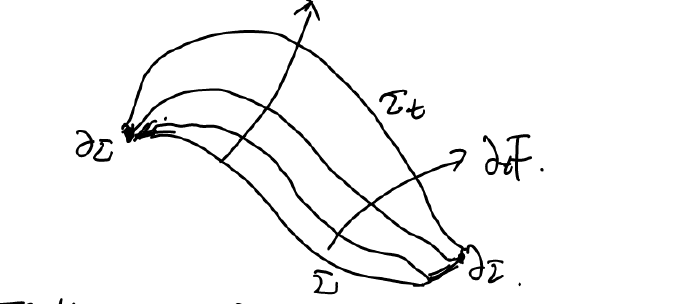
\includegraphics[scale=0.5]{images/variation.png}
	\caption{}
	\label{variation_p}
\end{figure}


\begin{remark}
    我们假设$\epsilon$足够小时, $F$是$\Sigma \times (-\epsilon,\epsilon)$到它的像之间的同胚. 选定$\Sigma$上的一组局部坐标系$(x^i)$. 以后我们将$\partial_t$与 $dF\partial_t$等同, 将$\partial_i$与$dF\partial_i$等同, 并分别记作$\partial_t F$与$\partial_i F$.
\end{remark}
设$\Sigma$上的度量为$g$, $\Sigma_t$上的度量记为 $g(t)$. 则$g_{ij}(t)=\inner{\partial_iF}{\partial_jF}$. 在这些记号下, 
\begin{equation}
    \Area(\Sigma_t)=\int_\Sigma \sqrt{\det g(t)}dx
\end{equation}
\begin{equation}
    \ddt \Area(\Sigma_t)=\int_\Sigma \ddt \sqrt{\det g(t)}dx
\end{equation}
现在我们来求面积的第一变分. 首先来证明一个引理.
\begin{lemma}
    设$A=[a_{ij}]$是 $n \times n$矩阵. 将$\det A$看作$n^2$个变量$(a_{ij})$的函数. 则$d\det A= A^{ij}da_{ij}$. $A^{ij}$是$A$的代数余子式.
\end{lemma}
\begin{proof}
    由行列式的拉普拉斯展开, 我们知道 $\forall j, \det A= \Sigma_{j}A^{ij}a_{ij}$. 注意到$A^{ij}$与${a_{ij}}$无关, 则有$\frac{\partial \det A}{\partial a_{ij}}=A^{ij}$.
\end{proof}
\begin{corollary} \label{det_jacobi}
    设$A_t=[a_{ij}(t)]$. 则$\ddt \det A_t=\det A_t \Tr(A_t^{-1}\ddt A_t)$.
\end{corollary}
现在, 固定一个点$p \in \Sigma$并选取$p$点处的测地坐标. 所有计算都将在点$p$处进行.
\begin{equation}
    \ddt \sqrt{\det g(t)}\mid_{t=0}=\Tr(g'(0))
\end{equation}
现在, 我们只需要计算$g'_{ij}(0)$即可. 根据定义, $g_{ij}(t)=\inner{\partial_iF}{\partial_jF}$. 对$t$求偏导, 则有
\begin{equation}
    \begin{split}
        \ddt g_{ij}(t)& =\nabla_{\partial_t F}\inner{\partial_iF}{\partial_jF} \\
                    & =\inner{\nabla_{\partial_t F}{\partial_iF}}{\partial_jF}+ \inner{\partial_iF}{\nabla_{\partial_tF}\partial_jF}
    \end{split}
\end{equation}
由于$\nabla_{\partial_tF}\partial_iF - \nabla_{\partial_iF} \partial_tF=[\partial_tF,\partial_iF]=dF[\partial_t,\partial_i]=0$, 则有

\begin{equation}
    \begin{split}
        \ddt g_{ij}(t) & =\inner{\nabla_{\partial_i F}{\partial_tF}}{\partial_jF}+ \inner{\partial_iF}{\nabla_{\partial_jF}\partial_tF}
    \end{split}
\end{equation}
因此,
\begin{equation}
    \Tr(g'(0))=\sum_i 2\inner{\nabla_{\partial_iF}\partial_tF}{\partial_iF} \mid_{t=0}=2\div_\Sigma \partial_tF\mid_{t=0}
\end{equation}
我们有
\begin{equation}
    \ddt \Area(\Sigma_t)\mid_{t=0}=\int_\Sigma \div_\Sigma \partial_t F
\end{equation}
而$\forall X \in TM$, 由于
\begin{equation}
    \nabla_{\partial_i}\inner{X^\perp}{\partial_j}=0=\inner{\nabla_{\partial_i}X^\perp}{\partial_j}+\inner{X^\perp}{\nabla_{\partial_i}\partial_j}
\end{equation}
以及 
\begin{equation}
    \div_\Sigma(X^\perp)=\sum_i\inner{\nabla_{\partial_i}X^\perp}{\partial_i}=-\sum_i\inner{X^\perp}{\nabla_{\partial_i}\partial_i}=-\inner{X^\perp}{\vec{H}}
\end{equation}
另外由于$\partial_tF|_{\partial \Sigma}=0$, 由散度定理可知
\begin{equation}
        \int_\Sigma \div_{\Sigma}(\partial_tF)^T =0.
\end{equation}
综上,我们有
\begin{equation}
    \begin{split}
        \ddt \Area(\Sigma_t)\mid_{t=0} & = \int_\Sigma \div_{\Sigma}(\partial_tF)^\perp + \int_\Sigma \div_{\Sigma}(\partial_tF)^T \\
        &=-\int_\Sigma\inner{\partial_tF}{\vec{H}}
    \end{split}
\end{equation}
因此, 若要使得曲面$\Sigma$的任意变分都不减小曲面的面积, 则$\Sigma$的平均曲率必定为0. 现在我们得到以下的定义:
\begin{definition}
    称$\Sigma^{n-1} \subset M^n$是极小曲面, 如果$H_\Sigma=0$.
\end{definition}
\section{曲面上的坐标函数}
设$\Sigma^{n-1} \subset \R^n$是光滑曲面. 设$\XX=(X^1,X^2,\cdots,X^n)$为$\R^n$上的坐标函数在$\Sigma$上的限制. $\XX$的一些性质如下.
\begin{enumerate}
    \item $\nabla_\Sigma \abs{\XX}^2=2\XX^T$,$\nabla_\Sigma \abs{\XX}=\frac{\XX^T}{\abs{\XX}}$.
    \item $\Delta_\Sigma \XX=(\Delta_\Sigma X^1, \Delta_\Sigma X^2, \cdots, \Delta_\Sigma X^n)= \vec{H}_\Sigma$.
    \item $\Delta_\Sigma \abs{\XX}^2 = 2(n-1)+2\inner{H}{\XX^\perp}$.%2H\abs{\XX^\perp}$.
\end{enumerate}
\begin{proof}
    性质(1)根据定义直接可以得到.
    \par 对于性质(2), 首先需要注意, 我们是在\textbf{对$\XX$的每个分量分别求导, 而不是求一个张量的Laplace}.  设$(\partial_i)$是$\R^n$的标准正交基. 我们注意到: 对于任意$Y=Y^i\partial_i \in \R^n$, $\nabla_Y\XX=Y^iX^j\nabla_{\partial_i}\partial_j+Y^i\partial_i(X^j)\partial_j=Y$. 取$T\Sigma$上的标准正交基$(e_i)$. 设$X^k$是$\XX$的第$k$个分量. 由于对于任意$Y \in T\Sigma$, $\nabla^\Sigma_Y X^k= \inner{\nabla^\Sigma X^k}{Y} = \inner{\nabla X^k}{Y} = Y(X^k)$, 则有
    \begin{equation}
        \begin{split}
            \Delta_\Sigma X^k &= \sum_i (\nabla^\Sigma_{e_i}\nabla^\Sigma_{e_i} X^k -\nabla^\Sigma_{\nabla^\Sigma_{e_i}e_i} X^k) \\
            &= \sum_i(e_ie_i X^k - (\nabla_{e_i}e_i)^T X^k).
            %&= \Tr A = \vec{H}
        \end{split}
    \end{equation}
    因此, 我们有
    \begin{equation}
        \begin{split}
            \Delta_\Sigma \XX  &= \sum_i(e_i(e_i \XX) - (\nabla_{e_i}e_i)^T \XX) \\
            &= \sum_i(\nabla_{e_i}e_i - (\nabla_{e_i}e_i)^T )\\
            &= \Tr A = \vec{H}.
        \end{split}
    \end{equation}
%    \begin{equation}
%        \begin{split}
%            \Delta_\Sigma \XX &= \sum_i (\nabla^\Sigma_{e_i}\nabla^\Sigma_{e_i}\XX-\nabla^\Sigma_{\nabla^\Sigma_{e_i}e_i}\XX) \\
%            &= \sum_i(\nabla_{e_i}e_i - (\nabla_{e_i}e_i)^T )\\
%            &= \Tr A = \vec{H}
%        \end{split}
%    \end{equation}
    \par 对于性质(3),
    \begin{equation}
        \Delta_\Sigma\abs{\XX}^2=\div_\Sigma(\nabla_\Sigma\abs{\XX}^2) = 2\div_\Sigma(\XX^T)=2\div_\Sigma(X)-2\div_\Sigma(X^\perp)
    \end{equation}
    分别计算这两项,则有
    \begin{equation}
        \div_\Sigma(\XX^\perp)=\sum_i \inner{\nabla_{e_i}X^\perp}{e_i}=-\sum_i\inner{X^\perp}{\nabla_{e_i}e_i}=-\inner{X^\perp}{\vec{H}}%=-\abs{X^\perp}H
    \end{equation}
    \begin{equation}
        \div_\Sigma(X)=\sum_i \inner{\nabla_{e_i}\XX}{e_i}=\sum_i\inner{e_i}{e_i}=n-1
    \end{equation}
    综合以上三个等式即可知性质(3).
\end{proof}
\begin{corollary} \label{coordinate_h}
    设$\Sigma^{n-1}\subset \R^n$. 则$\Sigma$是极小曲面当且仅当$\R^n$中的坐标函数在$\Sigma$上是调和的($\Sigma$上的度量继承自$\R^n$).
\end{corollary}
\begin{proof}
    性质(2)的直接推论.
\end{proof}
\begin{corollary}
    设$\Sigma^{n-1}\subset \R^n$是带有边界的极小曲面. 则$\Sigma \subset Conv(\partial\Sigma)$. Conv指的是集合的凸包.
\end{corollary}
\begin{proof}
    $\forall \vec{v} \subset \mathbb{S}^{n-1}$, 记$P_{\vec{v},a}=\{x\in \R^n\mid \inner{x}{\vec{v}} \le a\}$. 设$u(x)=\inner{x}{\vec{v}}$, 则$u(x)$是$\Sigma$上的调和函数. 因此, $u$的最大值只能在$\partial \Sigma$上取到. 若$\partial \Sigma \subset P_{\vec{v},a} $, 则 $\forall x \in \partial \Sigma$, $u(x) \le a$, 因此, $\forall x \in \Sigma$, $u(x) \le a$. 即, $\Sigma \subset P_{\vec{v},a}$. 证毕.
\end{proof}
\section{Schwartz反射}
由于推论\eqref{coordinate_h}, 极小曲面有许多性质跟调和函数非常相似(实际上极小曲面也是调和映射). 非常重要的一个应用便是Schwartz反射原理.
\begin{proposition} \label{min_reflection}
    设$\Sigma \subset \R^3$是极小曲面. 设$\Gamma \subset \partial \Sigma$是一段直线段. 设$\Sigma$有关直线$\Gamma$的对称反射的像为$\Sigma'$. 则$\Sigma \cup \Sigma'$是极小曲面.
\end{proposition}
   
\begin{figure}[h]
	\centering
	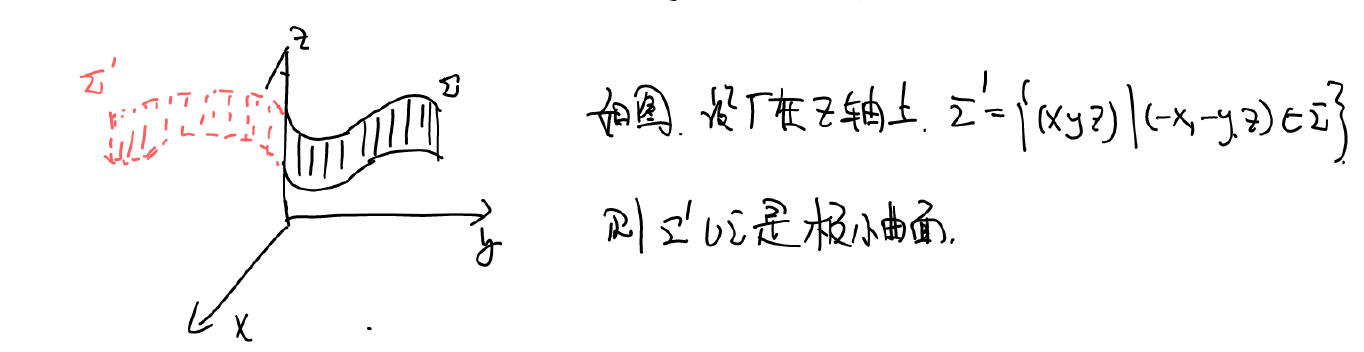
\includegraphics[scale=0.5]{images/reflection1.png}
	\caption{}
	\label{reflection1}
\end{figure}

\begin{lemma}
    设$\mathbb{D}$为单位圆盘, $\mathbb{D}^+,\mathbb{D}^-$为上半/下半单位圆盘. 设$u: \mathbb{D}^+ \to \R$是调和函数, 且在$x-$轴上, $u\eq 0$. 在$\mathbb{D}$上定义
    \begin{equation}
        \tilde{u}(x,y)= \left\{
            \begin{aligned}
                &u(x,y), (x,y) \in \mathbb{D}^+.\\
                &-u(x,-y), (x,y) \in \mathbb{D}^-.
            \end{aligned}
        \right.
    \end{equation}
    则$\tilde{u}$是$\mathbb{D}$上的调和函数.
\end{lemma}
\begin{proof}
    显然, $\tilde{u}$连续且在$\mathbb{D}^+,\mathbb{D}^-$内部都是调和的, 我们只需要考虑$\tilde{u}$在$x-$轴附近的行为. $\forall x_0 \in x-axis$, 取$B_r(x_0) \subset \mathbb{D}$. 解方程
    \begin{equation}
        \left\{
            \begin{aligned}
                &\Delta v=0, x \in B_r\\
                & v|_{\partial B_r(x_0)}=0
            \end{aligned}
        \right.
    \end{equation}
    方程的可解性由Poisson积分给出,在复坐标$z=x+iy$下
    \begin{equation}
        v(a)=\frac{1}{2\pi} \int_{\abs{z-x_0}=r} \frac{r^2-\abs{a-x_0}^2}{\abs{z-a}^2}\tilde{u}(z)ds
    \end{equation}
    由于$\forall z \in \partial B_r(x_0), \tilde{u}(z)=-\tilde{u}(\bar{z})$. 则$\forall a\in B_r, v(a)=-v(\bar{a})$. 则在$x-$轴上, $v\eq 0$. 因此, $v|_{\partial{B_r^+}}=\tilde{u}|_{\partial{B_r^+}}$, $v|_{\partial{B_r^-}}=\tilde{u}|_{\partial{B_r^-}}$. 由最大值原理可知在$B_r$上, $\tilde{u}=v$. 因此, $\tilde{u}$是调和的.
\end{proof}
\begin{lemma}[等温坐标的存在性]
    设$(M^2, g)$是二维黎曼流形, 则存在$M^2$上的一组坐标卡$\{z=x+iy\}$, 使得在这组坐标下, $g=\lambda^2\abs{dz}^2$, 并且这组坐标下的坐标变换是全纯的.
\end{lemma}

\begin{figure}[h]
	\centering
	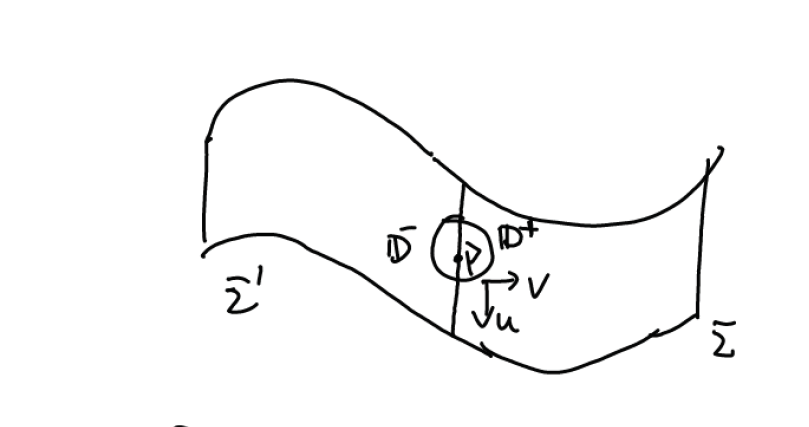
\includegraphics[scale=0.5]{images/reflection2.png}
	\caption{}
	\label{reflection2}
\end{figure}
\begin{proof}[命题\eqref{min_reflection}的证明]
    取$\Sigma$上的等温坐标, 显然地, $\Sigma$上的等温坐标经反射后得到$\Sigma'$上的等温坐标. 将$z-$轴看作是$\mathbb{C}={w=u+iv}$上的$u-$轴. 将$B_r(p)\cap \Sigma$看作 $\mathbb{D}^+$, 将$B_r(p) \cap \Sigma'$看作$\mathbb{D}^-$. 现在, 利用调和函数的反射性质可知, 在$\Sigma \cap \Sigma'$上, $x,y$坐标都是调和的. 我们只需要说明$z-$坐标也是调和的即可. 由$\Sigma'$的构造可知, $z(u,v)=z(u,-v)$. 设$\vec{n}$是$B_r\cap \Sigma$在$z-$轴上的单位法向, 则$\frac{\partial z}{\vec{n}}= \partial_v{z}=0$. 于是, $z$满足 $\partial_v z(u,v)=-\partial_v z(u,-v)$. 由Schwzrtz 反射可知, $z_v$是调和函数, 则$z$是调和的. 
\end{proof}
\begin{remark}
    由此可见, 极小曲面上包含直线是非常强的条件. Schwartz反射的一类非常重要的应用是当极小曲面的边界上包含两条平行的直线的情况下.  这个时候我们可以做无穷多次反射得到一个周期的极小曲面.
\end{remark}
\begin{proposition} \label{conformal_im}
    设 $X(u,v): \mathbb{D} \to \R^3$是共形浸入. 则$\Sigma = X(\mathbb{D})$是极小曲面当且仅当$X$的每个分量是调和函数.
\end{proposition}
\begin{proof}
    由于$X$是共形浸入, 则在$\Sigma$上的度量在$z=u+iv$坐标下可以表示为$\lambda^2\abs{dz}^2$的形式, 而$\Delta_\Sigma X= \frac{4}{\lambda^2} \Delta X=0$.
\end{proof}
\begin{remark}
    $\Sigma\subset \R^3$是极小曲面当且仅当$\R^3$中的坐标函数在$\Sigma$上的限制是调和的, 这里$\Sigma$上必须是继承自$\R^3$上的度量. 命题 \eqref{conformal_im}中的共形浸入的条件是必不可少的, 比如, 设$X:\mathbb{D}\to \R^3, X(u,v)=(u,v,uv)$. 显然地, $\Delta X=0$. 但是$X(\mathbb{D})$不是极小曲面.
\end{remark}
\section{单调性公式}
\begin{proposition}[余面积公式]
    设$\Sigma^{n-1}\subset \R^n$是光滑曲面.  设$h: \Sigma \to \R$是Lipschitz, proper(紧集的原像为紧集)映射.  则$\forall f \in L^1_{\loc}(\Sigma)$, 成立
    \begin{equation}
        \int_{h < t} f \abs{\nabla_\Sigma h}dH^{n-1}=\int^t_{-\infty} \int_{h=r}f dH^{n-2}dr
    \end{equation}
\end{proposition}
\begin{proposition}
设$\Sigma^{n-1}\subset \R^n$是光滑曲面. 设$t>s$且$B_t(p) \cap \partial \Sigma =\emptyset$. 设$f \in C^1(\Sigma)$, $H$是$\Sigma$的平均曲率.  则有    
\begin{equation}
    \begin{split}
        &\frac{1}{t^{n-1}}\int_{\Sigma\cap B_t} f dH^{n-1}-\frac{1}{s^{n-1}}\int_{\Sigma\cap B_s} f dH^{n-1} \\
        =& \int_{\Sigma \cap (B_t-B_s)} f \frac{\abs{(x-p)^\perp}^2}{\abs{x-p}^{n+1}} \\
        &+\frac{1}{2}\int^t_s \frac{1}{r^n}\int_{\Sigma\cap B_r}(r^2-\abs{x-p}^2)\Delta_{\Sigma}f+2f\inner{\vec{H}}{(x-p)^\perp}dH^{n-1}dr
    \end{split}
\end{equation}
\end{proposition}
\begin{proof}
     记$I(r)=\frac{1}{r^{n-1}}\int_{\Sigma\cap B_r} f$. 不失一般性, 设$p=0$. 对$I(r)$求导,则有
     \begin{equation} \label{ddr}
        \ddr I(r)=-(n-1)\frac{1}{r^n}\int_{\Sigma \cap B_r} f + \frac{1}{r^{n-1}}\ddr \int_{\Sigma \cap B_r} f
     \end{equation}
     我们分别计算上式右侧的两项. 首先来计算第二项. 设$f=g\frac{\abs{x^T}}{\abs{x}}=g\abs{\nabla_\Sigma \abs{x}}$. 则由余面积公式(取$h=\abs{x}$),
     \begin{equation}
        \begin{split}
            \int_{\Sigma \cap B_r} f = \int_{\{\abs{x} < r\}\cap \Sigma }g \abs{\nabla_\Sigma \abs{x}} &= \int^r_{-\infty} \int_{\{\abs{x}=\rho\} \cap \Sigma} g dH^{n-2}d\rho 
            %&= \int^r_{-\infty}\int_{\partial B_\rho \cap \Sigma} g
        \end{split}
     \end{equation}
     因此, 
     \begin{equation} \label{ddr2}
        \ddr \int_{\Sigma \cap B_r} f= \int_{\partial B_r \cap \Sigma} f \frac{\abs{x}}{\abs{x^T}} =r\int_{\partial B_r\cap \Sigma} f \frac{1}{\abs{x^T}}.
     \end{equation}
     设$\vec{n}$是$B_r\cap \Sigma$在$\partial B_r\cap \Sigma$上的单位法向. 容易验证 $\inner{x^T}{\vec{n}}= \abs{x^T}$.  现在,我们来计算第一项. 由$\Delta_\Sigma \abs{x}^2=2(n-1)+2\inner{\vec{H}}{x^\perp}$及分部积分公式可知,
     \begin{equation} \label{ddr1}
        \begin{split}
            2(n-1)\int_{\Sigma \cap B_r}f =&\int_{\Sigma \cap B_r}f \Delta_{\Sigma}\abs{x}^2-2\int_{\Sigma \cap B_r} f\inner{\vec{H}}{x^\perp} \\
            =& \int_{\Sigma \cap B_r}\abs{x}^2 \Delta_\Sigma f + 2\int_{\partial B_r\cap \Sigma}f\inner{\vec{n}}{x^T}  \\
            &- \int_{\partial B_r \cap \Sigma}\abs{x}^2 \inner{\vec{n}}{\nabla_{\Sigma}f}-2\int_{\Sigma \cap B_r} f\inner{\vec{H}}{x^\perp}\\
            &=I+II+III+IV
        \end{split}
     \end{equation}
     现在,在等式\eqref{ddr1}中,
     \begin{equation}
        II=2\int_{\partial B_r\cap \Sigma}f\abs{x^T}.
     \end{equation}
     \begin{equation}
        III=-r^2\int_{\partial B_r\cap \Sigma} \inner{\vec{n}}{\nabla_\Sigma} =-r^2\int_{{B_r} \cap \Sigma} \Delta_{\Sigma}f.
     \end{equation}
     现在, 将\eqref{ddr1}及\eqref{ddr2}代入到\eqref{ddr}中, 则有
     \begin{equation}\label{ddr_i}
        \begin{split}
            \ddr I(r) =& -\frac{1}{2r^n}\int_{\Sigma \cap B_r}\abs{x}^2 \Delta_\Sigma f - \frac{1}{r^n} \int_{\partial B_r\cap \Sigma} f \abs{x^T} + \frac{1}{2r^{n-2}} \int_{B_r\cap \Sigma} \Delta_\Sigma f \\
            &+ \frac{1}{r^n} \int_{\Sigma \cap B_r fH\abs{x^\perp}} + \frac{1}{r^{n-2}} \int_{\partial B_r \cap \Sigma} \frac{f}{\abs{x^T}} \\
            =& \frac{1}{2r^n} \int_{\Sigma \cap B_r}(\Delta_\Sigma f(r^2-\abs{x}^2) + 2\inner{\vec{H}}{x^\perp}) + \frac{1}{r^n}\int_{\partial B_r\cap \Sigma} f \frac{\abs{x^\perp}^2}{\abs{x^T}}
        \end{split}
     \end{equation}
     再次利用余面积公式以及$\abs{\nabla^\Sigma\abs{x}}=\frac{\abs{x^T}}{\abs{x}}$, 上式右侧第二项的积分为
     \begin{equation} \label{ddr_i2}
        \begin{split}
            \int^t_s \frac{1}{r^n} \int_{\partial B_r \cap \Sigma} f \frac{\abs{x^\perp}^2}{\abs{x^T}^2} &= \int^t_s \int_{\{\abs{x} = r\}\cap \Sigma} f  \frac{\abs{x^\perp}^2}{\abs{x^T}} \frac{1}{\abs{x}^n} \\
            &= \int_{\{s<\abs{x}<t\}\cap \Sigma } f \frac{\abs{x^\perp}^2}{\abs{x^T}}\frac{1}{\abs{x}^n}\abs{\nabla_\Sigma\abs{x}} \\
            &=\int_{(B_t-B_s)\cap \Sigma} f \frac{\abs{x^\perp}^2}{\abs{x}^{n+1}}
        \end{split}
     \end{equation}
     在等式$\eqref{ddr_i}$两侧取积分, 并将\eqref{ddr_i2}代入即可得到单调性公式.
\end{proof}
\begin{corollary}
    设$\Sigma^{n-1} \subset \R^n$是极小曲面. $x_0 \subset \Sigma$, $B_s(x_0) \cap \partial \Sigma = \emptyset$. 设$f \in C^\infty(\Sigma)$且 $f \ge 0, \Delta_{\Sigma}f \ge -\lambda s^2 f$, 则有
    \begin{equation}
        f(x_0) \le e^{\frac{\lambda}{2}}\frac{\int_{B_s\cap \Sigma}f}{\abs{B_s\subset \R^{n-1}}}
    \end{equation}
\end{corollary}
\begin{proof}
    设$g(t)=\frac{1}{t^{n-1}}\int_{B_t\cap \Sigma}f, t\le s$. 则由单调性公式, 
    \begin{equation}
        \begin{split}
            g'(t) &\ge \frac{1}{2}\frac{1}{t^n}\int_{B_t\cap \Sigma}(t^2-\abs{x}^2)\Delta_\Sigma f \\
            &\ge -\frac{\lambda}{2}\frac{1}{t^{n-2}s^2}\int_{B_t\cap \Sigma}f = -\frac{\lambda}{2}\frac{t}{s^2}g(t).
        \end{split}
    \end{equation}
    于是有,
    \begin{equation}
        \frac{g'(t)}{g(t)} \ge - \frac{\lambda}{2s^2}t\ge -\frac{\lambda}{2s}
    \end{equation}
    而这等价于: $\ddt (e^{\frac{\lambda t}{2s}g(t)}) \ge 0$. 证毕.
\end{proof}
\section{Gauss映射}
设$\Sigma \subset \R^3$是光滑曲面. 设$\vec{n}$为其单位法向. 由于在$\R^3$中, $\vec{n}$可以看作$\S^2$上的点, 我们可以得到映射$\N:\Sigma \S^2, \N(p)=\vec{n}(p), p \in \Sigma$. 称$\N$为曲面 $\Sigma$的Gauss映射.
\begin{proposition}
    设$p \in \Sigma$, 则$T_{\N(p)}\S^2= T_p\Sigma$.
\end{proposition}
\begin{proof}
    $T_{\N(p)}\S^2=\{x\in \R^n\mid \inner{x}{\N(p)}=\inner{x}{\vec{n}}\}$.
\end{proof}
\begin{proposition}
    $\forall X, Y \in T_p\Sigma$, 有等式: 
    \begin{equation}
        \inner{II(X,Y)}{\vec{n}}=-\inner{\nabla_X\vec{n}}{Y}=-\inner{d\N X}{Y}.
    \end{equation}
\end{proposition}
\begin{proof}
    由于$\inner{\vec{n}}{Y}=0$, 则有 $\inner{\nabla_XY}{\vec{n}}=-\inner{Y}{\nabla_X\vec{n}}$. 
    \par 第二个等式是因为 $\nabla_X\vec{n}=(\nabla \vec{})X=d\N X$, 即是欧氏空间中的方向导数.
\end{proof}
\begin{proposition} \label{gauss_anticonformal}
    设$\Sigma \subset \R^3$是光滑曲面. 则$\Sigma$是极小曲面当且仅当其Gauss映射是反共形的($\S^2$上取由外单位法向所给定的定向). 反共形指的是保持角度大小而不保持方向.
\end{proposition}
\begin{proof}
    固定点$p \in \Sigma$. 由于$II$是对称的, 则存在局部标架$\{e_i\}$, 使得在$p$点处, $II e_1=\lambda_1 e_1$, $II e_2=\lambda_2 e_2$. (这里, $\lambda_i,e_i$分别被称作曲面$\Sigma$的主曲率与主曲率方向). 现在,我们有
    \begin{equation}
        \inner{d\N e_i}{d\N e_j}= \inner{\nabla_{e_i}\vec{n}}{\nabla_{e_j}\vec{n}} \lambda_i\lambda_j\inner{e_i}{e_j}
    \end{equation}
    显然地,  $dN=diag(\lambda_1,\lambda_2)$是反共形的当且仅当$\lambda_1+\lambda_2=0$, 当且仅当$\Sigma$是极小曲面.
\end{proof}
\begin{proposition}
    设$\Sigma \subset \R^3$是极小曲面. $\N$为其Gauss映射. $d\Sigma, \omega$分别为$\Sigma, \S^2$上的面积形式, 设$N^*\omega$为其拉回. 则有
    \begin{equation}
        \abs{II}^2d\Sigma= -2N^*\omega.
    \end{equation}
\end{proposition}
\begin{proof}
    如是同在命题\eqref{gauss_anticonformal}的证明中选择$\{e_i\}$. 设$\{e^{*i}\}$为其对偶标架. 由于$\lambda_1+\lambda_2=0$, 则
    \begin{equation}
        \abs{II}^2d\Sigma=(\lambda_1^2+\lambda_2^2)e^{*1}\wedge e^{*2}=-2\lambda_1\lambda_2 e^{*1}\wedge e^{*2}.
    \end{equation}
    而由于$d\N=diag(\lambda_1,\lambda_2)$, 则 $\abs{II}^2d\Sigma=-2N^* e^{*1} \wedge e^{*2}$.
\end{proof}
\section{Bernstein定理}
\begin{proposition} \label{caccio}
    设$u: \Omega \subset \R^2 \to \R$满足MSE. 设$\Sigma=\G(u)$. 设$\phi \in Lip(\Sigma)$且$\phi$具有紧支集, 则
    \begin{equation}
        \int_{\Sigma}\abs{II}^2\phi^2 \le C\int_\Sigma \abs{\nabla_{\Sigma}\phi}^2
    \end{equation}
    这里,  $C$是万有常数.
\end{proposition}
\begin{proof}
    显然地, $\N(\Sigma) \subset \S^2_+$. 设$\omega$是 $\S^2$上的面积形式. 由于$\S^2_+$是单连通的, 则存在$1-$形式$\alpha$使得  $\Omega=d\alpha$. 于是有 
    \begin{equation}
        \abs{II}^2d\Sigma=-2\N^*\omega=-2\N^*d\alpha=-2d(\N*\alpha)
    \end{equation}
    由于$\forall 1-$形式$\beta$ , $d(\phi^2\beta)=\phi^2\beta+2\phi d\phi\wedge\beta$, 再由Stokes公式
    \begin{equation}
        \begin{split}
            \int_\Sigma \abs{II}^2\phi^2 = -2 \int_\Sigma \phi^2 d(\N^*\alpha) &=-2\int_\Sigma d(\phi^2\N^*\alpha)+4\int_\Sigma \phi d\phi\wedge N^*\alpha\\
            &= 4\int_\Sigma  \phi d\phi\wedge N^*\alpha
        \end{split}
    \end{equation}
    在局部标架下, $\phi=\phi_i e^{*i}, N^*=diag(\lambda_1,\lambda_2), \alpha=\alpha_i e^{*i}$. 因此, 若设 $d\phi\wedge \N^*\alpha= f(x)d\Sigma$, 则 $\abs{f} \le C_\alpha \abs{\nabla_\Sigma}\abs{II}$. 于是有
    \begin{equation}
        \begin{split}
            \int_\Sigma \abs{II}^2\phi^2 &\le C_\alpha \abs{A}\abs{\phi} \abs{\nabla_\Sigma \phi} \\
            & le C_\alpha(\epsilon \int_\Sigma \abs{II}^2\phi^2 + \frac{1}{\epsilon}\int_\Sigma  \abs{\nabla_\Sigma \phi}^2 \\
        \end{split}
    \end{equation}
    取$\epsilon$使得 $\epsilon C_\alpha=\frac{1}{2}$即可.
\end{proof}
\begin{theorem}
    设$u: \R^2 \to \R$在全平面上满足MSE.  记$\Sigma=\G(u)$. 则$u$是仿射函数, 或者等价地, $\Sigma$是平面.
\end{theorem}
\begin{proof}
    我们首先说明, 如果下面的断言成立, 则$u$是仿射.
    \begin{claim}
        $\forall k >0$,存在$\phi_k \in Lip(\Sigma)$使得  $\phi_k|_{B_k \cap \Sigma}=1$, $\phi_k$有紧支集 且$ \int_\Sigma \abs{\nabla_\Sigma \phi_k}^2 \to 0$.
    \end{claim}
    若断言成立, 那么由不等式\eqref{caccio}可知, $\int_{\Sigma\cap B_k} \abs{II}^2 \le \int_\Sigma \abs{\nabla_\Sigma \phi_k}^2 \to 0$. 则$II\eq 0$. 因此$\Sigma$为平面. 
    \par 现在我们来证明断言成立. $\forall k>0$, 定义
    \begin{equation}
        \phi_k(x)=\left\{
            \begin{aligned}
                &1, \abs{x} < k, \\
                &1-\frac{\log\abs{x}-\log k}{\log k}, k \le \abs{x} \le k^2,\\
                &0, \abs{x} > k^2
            \end{aligned}
        \right.
    \end{equation}
    记$R_{s,t}=B_t-B_s$为环域. 将$R_{k,k^2}$分解为若干环域的并 
    \begin{equation}
        R_{k,k^2}=\cup_{i=0}^{\log k} R_{2^ik,2^{i+1}k}.
    \end{equation}
    直接计算可知, 在环域$R_{2^ik,2^{i+1}k}$上,
    \begin{equation}
        \abs{\nabla_\Sigma \phi} \le \abs{\nabla \phi} \le \frac{1}{\log k} \frac{1}{\abs{x}}
    \end{equation}
    以及
    \begin{equation}
        \abs{R_{2^ik,2^{i+1}k} \cap \Sigma } \le C 2^{2i}k^2. 
    \end{equation}
    于是,我们有
    \begin{equation}
        \int_\Sigma \abs{\nabla_\Sigma \phi_k}^2 \le C\sum_{i=0}^{\log k} 2^{2i}k^22\frac{1}{(\log k)^2} \frac{1}{2^{2i}k^2} \le C\frac{1}{\log k} \to 0.
    \end{equation}
    断言得证.
\end{proof}
\section{Weierstrass表示}
\section{第二变分公式与稳定性}